\documentclass[10pt]{article}
\usepackage{fullpage}
\usepackage{graphicx}
\usepackage{url}
\usepackage{hyperref}
\usepackage{rotating}
\usepackage{color}
\usepackage{fancybox}
\usepackage{fancyvrb}
\usepackage[T1]{fontenc}

%opening
\title{CMSC 23300 -- Networks and Distributed Systems\\{\large Project 1: Internet Relay Chat}}
\date{}

\newcommand{\chirc}{$\chi$\textsf{irc} }

\newcommand{\RFC}[1]{\href{http://tools.ietf.org/html/rfc#1}{[RFC#1]}}
\newcommand{\RFCsection}[2]{\href{http://tools.ietf.org/html/rfc#1\#section-#2}{[RFC#1 \textsection #2]}}

\newcommand{\points}[1]{{\sffamily\mdseries\guillemotleft #1 points\guillemotright{}}}

\definecolor{backgroundgray}{gray}{0.9}

\fvset{tabsize=2}
\DefineVerbatimEnvironment{VerbExample}{BVerbatim}{boxwidth=0.9\textwidth,fontsize=\footnotesize,samepage=true,commandchars=\\\{\}}
\newenvironment{example}%
{\VerbatimEnvironment\begin{Sbox}\begin{VerbExample}}%
{\end{VerbExample}\end{Sbox}\setlength{\fboxsep}{8pt}\begin{center}\fcolorbox{black}{backgroundgray}{\TheSbox}\end{center}}

\begin{document}
\pagestyle{empty}
\maketitle

\section{Introduction}

In this project, you will implement a simple Internet Relay Chat (IRC) server called \chirc. This project has three goals:

\begin{enumerate}
 \item To provide a refresher of socket and concurrent programming covered in CMSC 15400.
 \item To implement a system that is (partially) compliant with an established network protocol specification.
 \item To allow you to become comfortable with high-level networking concepts before we move on to the lower-level concepts in this course.
\end{enumerate}

This project is divided into three parts. The first part is meant as a relatively short warmup exercise, and you should be able to do it just by applying what you learned about network sockets in CMSC 15400. The other two parts are more complex, but should still be doable if you've taken CMSC 15400 (we will, nonetheless, be covering some additional topics in the first lectures that will come in handy to do this project).

This document is divided into three parts: Sections \ref{sec:irc} through \ref{sec:examples} provide an overview of IRC and provide several examples of valid IRC communications; Sections \ref{sec:code} to \ref{sec:repo} describe how to get the \chirc code, and how to build it and upload it to your code repository; finally, Sections \ref{sec:grading} to \ref{sec:proj1c} describe how the project will be graded, and the specific requirements of the three parts the project is divided into.

\section{Internet Relay Chat}
\label{sec:irc}

IRC is one of the earliest network protocols for text messaging and multi-participant chatting. It was created in 1988 and, despite the emergence of more sophisticated messaging protocols (including open standards like XMPP and SIP/SIMPLE, and proprietary protocols such as Microsoft's MSNP, AOL's OSCAR, and Skype), IRC remains a popular standard and still sees heavy use in certain communities, specially the open source software community.

\begin{figure}
\begin{center}
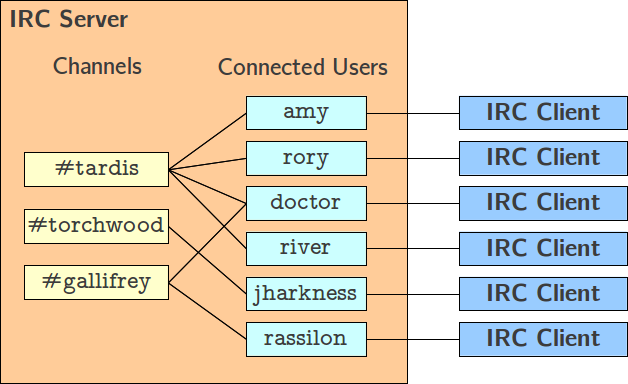
\includegraphics[width=0.7\textwidth]{architecture1.png}
\caption{Basic IRC architecture}
\end{center}
\label{fig:architecture1}
\end{figure}

The basic architecture of IRC, shown in Figure~\ref{fig:architecture1}, is fairly straightforward. In the simplest case, there is a single \emph{IRC server} to which multiple \emph{IRC clients} can connect to. An IRC client connects to the server with a specific identity. Most notably, each client must choose a unique \emph{nickname}, or ``nick''. Once a client is connected, it can communicate one-to-one with other users. Additionally, clients can run commands to query the server's state (e.g., to obtain a list of connected users, or to obtain additional details about a specific nick). IRC also supports the creation of chat rooms called \emph{channels} for one-to-many communication. Users can join channels and send messages to the channel; these messages will, in turn, be sent to every user in the channel.

\begin{figure}
\begin{center}
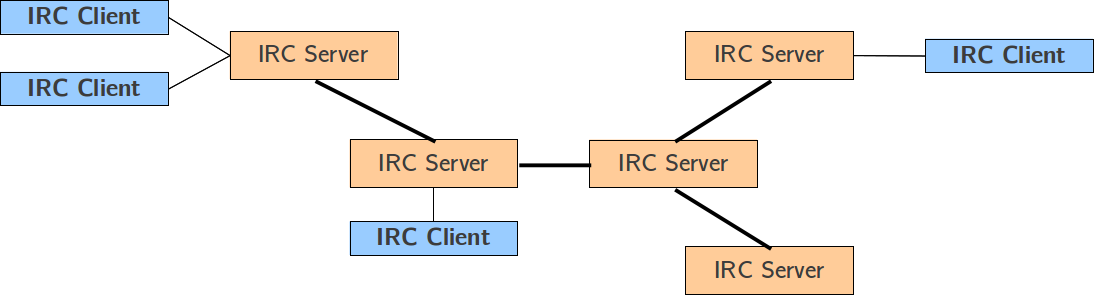
\includegraphics[width=1\textwidth]{architecture2.png}
\caption{Multi-server IRC architecture}
\end{center}
\label{fig:architecture2}
\end{figure}

IRC also supports the formation of \emph{server networks}, where multiple servers form a tree of connections to support more clients and provide greater capacity. Servers in the same network share information about local events (e.g., a new client connects, a user connected to a given server joins a channel, etc.) so that all servers will have a copy of the same global state. In this project, we will only consider the case where there is a single IRC server.


\section{The IRC Protocol}
\label{sec:protocol}

The IRC protocol used by IRC servers and clients is a text-based TCP protocol. Originally specified in 1993 \RFC{1459}, it was subsequently specified in more detail in 2000 through the following RFCs:

\begin{itemize}
\item \RFC{2810} \textbf{Internet Relay Chat: Architecture}. This document describes the overall architecture of IRC.
\item \RFC{2811} \textbf{Internet Relay Chat: Channel Management}. This document describes how channels are managed in IRC.
\item \RFC{2812} \textbf{Internet Relay Chat: Client Protocol}. This document describes the protocol used between IRC clients and servers (sometimes referred to as the ``client-server'' protocol)
\item \RFC{2813} \textbf{Internet Relay Chat: Server Protocol}. This document describes the ``server-server'' protocol used between IRC servers in the same network.
\end{itemize}

You are not expected to read all of these documents. More specifically:

\begin{itemize}
\item We recommend you do read all of \RFC{2810}, as it will give you a good sense of what the IRC architecture looks like. You may want to give it a cursory read at first, and revisit it as you become more familiar with the finer points of the IRC protocol.
\item In Project 1b you will implement a subset of \RFC{2812}. We suggest you read \RFCsection{2812}{1} and \RFCsection{2812}{2}. For the remainder of the RFC, you should only read the sections relevant to the parts of the IRC protocol you will be implementing.
\item In Project 1c you will implement a subset of the functionality described in \RFC{2811}, which will require implementing additional parts of \RFC{2812}. We suggest you hold off on reading \RFC{2811} until we reach Project 1c; if you do want to read the introductory sections, take into account that we will only be supporting ``standard channels'' in the ``\#'' namespace, and that we will not be supporting server networks.
\item We will not be implementing any part of \RFC{2813}.
\end{itemize}

Finally, you should take into account that, although IRC has an official specification, most IRC servers and clients do not conform to these RFCs. Most (if not all) servers do not implement the full specification (and even contradict it in some cases), and there are many features that are unique to specific implementations. In this project, we will produce an implementation that is partially compliant with these RFCs, and sufficiently compliant to work with some of the main IRC clients currently available.

In the remainder of this section, we will see an overview of the message format used in IRC. Then, in the next section, we will see several example communications (involving multiple messages between a client and a server).

\subsection{Message format}

IRC clients and servers communicate by sending plain ASCII \emph{messages} to each other over TCP. The format of these messages is described in \RFCsection{2812}{2.3}, and can be summarized thusly:

\begin{itemize}
\item The IRC protocol is a \emph{text-based} protocol, meaning that messages are encoded in plain ASCII. Although not as efficient as a pure binary format, this has the advantage of being fairly human-readable, and easy to debug just by reading the verbatim messages exchanged between clients and servers.
\item A single message is a string of characters with a maximum length of 512 characters. The end of the string is denoted by a CR-LF (Carriage Return - Line Feed) pair (i.e., ``\verb+\r\n+''). There is no null terminator. The 512 character limit includes this delimiter, meaning that a message only has space for 510 useful characters.
\item The IRC specification includes no provisions for supporting messages longer than 512 characters, although many servers and clients support non-standard solutions (including ignoring the 512 limit altogether). In our implementation, any message with more than 510 characters (not counting the delimiter) will be truncated, with the last two characters replaced with ``\verb+\r\n+''.
\item A message contains at least two parts: the command and the command parameters. There may be at most 15 parameters. The command and the parameters are all separated by a single ASCII space character. The following are examples of valid IRC messages:

\begin{example}
NICK amy
WHOIS doctor
MODE amy +o
JOIN #tardis
QUIT
\end{example}

\item When the last parameter is prefixed with a colon character, the value of that parameter will be the remainder of the message (including space characters). The following are examples of valid IRC messages with a ``long parameter'':

\begin{example}
PRIVMSG rory :Hey Rory...
PRIVMSG #cmsc23300 :Hello everybody
QUIT :Done for the day, leaving
\end{example}

\item Some messages also include a \emph{prefix} before the command and the command parameters. The presence of a prefix is indicated with a single leading colon character. The prefix is used to indicate the \emph{origin} of the message. For example, when a user sends a message to a channel, the server will forward that message to all the user in the channel, and will include a prefix to specify the user that sent that message originally. We will explain the use of prefixes in more detail in the next section. 

The following are examples of valid IRC messages with prefixes:

\begin{example}
:borja!borja@polaris.cs.uchicago.edu PRIVMSG #cmsc23300 :Hello everybody
:doctor!doctor@baz.example.org QUIT :Done for the day, leaving
\end{example}
\end{itemize}

\subsection{Replies}

The IRC protocol includes a special type of message called a \emph{reply}. When a client sends a command to a server, the server will send a reply (except in a few special commands where a reply should not be expected). Replies are used to acknowledge that a command was processed correctly, to indicate errors, or to provide information when the command performs a server query (e.g., asking for the list of users or channels).

A reply is a message with the following characteristics:

\begin{itemize}
\item It always includes a prefix.
\item The command will be a three-digit code. The full list of possible replies is specified in \RFCsection{2812}{5}.
\item The first parameter is always the target of the reply, typically a nick.
\end{itemize}

The following are examples of valid IRC replies:

\begin{example}
:irc.example.com 001 borja :Welcome to the Internet Relay Network borja!borja@polaris.cs.uchicago.edu
:irc.example.com 433 * borja :Nickname is already in use.
:irc.example.org 332 borja #cmsc23300 :A channel for CMSC 23300 students
\end{example}

\section{Example communications}
\label{sec:examples}

In this section, we will describe three example IRC communications. Before diving into the IRC RFCs, we suggest you read through these examples to get a better sense for what a typical conversation between an IRC client and server looks like. These examples will also serve to clarify the format of messages, prefixes, and replies.

\subsection{Logging into an IRC server}
\label{sec:logging}


\begin{figure}
\begin{center}
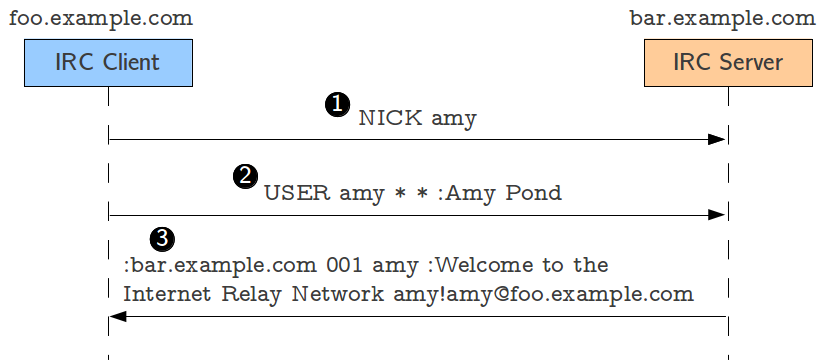
\includegraphics[width=0.7\textwidth]{connect.png}
\caption{Connecting to an IRC server}
\label{fig:connect}
\end{center}
\end{figure}

When an IRC client connects to an IRC server, it must first \emph{register} its connection. This is done by sending two messages: \texttt{NICK} and \texttt{USER} (messages 1 and 2 in Figure~\ref{fig:connect}). \texttt{NICK} specifies the user's nick (\texttt{amy} in this case), and \texttt{USER} provides additional information about the user. More specifically, \texttt{USER} specifies the user's \emph{username} (\texttt{amy}) and the user's \emph{full name} (\texttt{Amy Pond}) (we will not be implementing the second and third parameters of \texttt{USER}). The username is typically obtained automatically by the IRC client based on the user's identity. For example, if you're logged into a UNIX machine as user \texttt{jrandom}, then most IRC clients will, by default, use that as your username. However, there is no requirement that your nick must match your username.

Assuming you've chosen a nick that is not already taken, the IRC server will send back a \texttt{RPL\_WELCOME} reply (which is assigned code \texttt{001}). This reply has the following components:

\begin{itemize}
\item \texttt{:bar.example.com}: The prefix. Remember that prefixes are used to indicate the origin of a message. Since this reply originates in server \texttt{bar.example.com}, the prefix simply includes that hostname. This may seem redundant, given that the client presumably already knows it is connected to that server; however, in IRC networks, a reply could originate in a server other than the one the client is connected to.
\item \texttt{001}: The numeric code for \texttt{RPL\_WELCOME}.
\item \texttt{amy}: The first parameter which, in reply messages, must always be the nick of the user this reply is intended for.
\item \texttt{:Welcome to the Internet Relay Network borja!borja$@$polaris.cs.uchicago.edu}: The second parameter. The content of this parameter is specified in \RFCsection{2812}{5}:

\begin{example}
       001    RPL_WELCOME
              "Welcome to the Internet Relay Network
               <nick>!<user>@<host>"
\end{example}

Notice how the specification of replies omits the first parameter, which is always the recipient of the reply. So, the specification lists the second and subsequent (if any) parameters.

One of the things sent back in the \texttt{RPL\_WELCOME} reply is the \emph{full client identifier} (\texttt{<nick>!<user>$@$<host>}), which is also used in other types of messages. It is composed of the nick as specified in the \texttt{NICK} command, the username as specified in the \texttt{USER}, and the client's hostname (if the server cannot resolve the client's hostname, the IP address is used).
\end{itemize}

\begin{figure}
\begin{center}
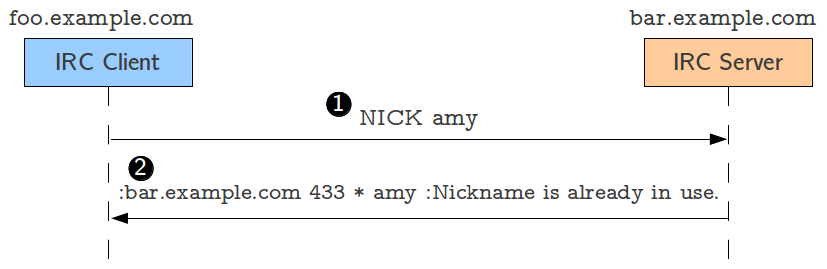
\includegraphics[width=0.7\textwidth]{duplicatenick.png}
\caption{Connecting to an IRC server when the chosen nick is taken.}
\label{fig:duplicatenick}
\end{center}
\end{figure}

Figure~\ref{fig:duplicatenick} shows a variant of the communication described above. If a user tries to register with a nick that is already taken, the server will send back a \texttt{ERR\_NICKNAMEINUSE} reply (code \texttt{433}). Notice how the parameters in this reply are slightly different:

\begin{itemize}
\item \texttt{*}: The first parameter should be the nick of the user this reply is intended for. However, since the user does not yet have a nick, the asterisk character is used instead.
\item \texttt{amy}: In the \texttt{ERR\_NICKNAMEINUSE} reply, the second parameter is the ``offending nick'' (i.e., the nick that could not be chosen, because it is already taken).
\item \texttt{:Nickname is already in use}: The third parameter simply includes a human readable description of the error. IRC clients will typically print these out verbatim.
\end{itemize}

So, notice how there is no uniform set of parameters sent back in all replies (other than the first parameter, which is always the recipient nick). When implementing a reply, you must consult \RFCsection{2812}{5} to determine exactly what you should be sending back in the reply.

\subsection{Messaging between users}
\label{sec:privmsg}

\begin{figure}
\begin{center}
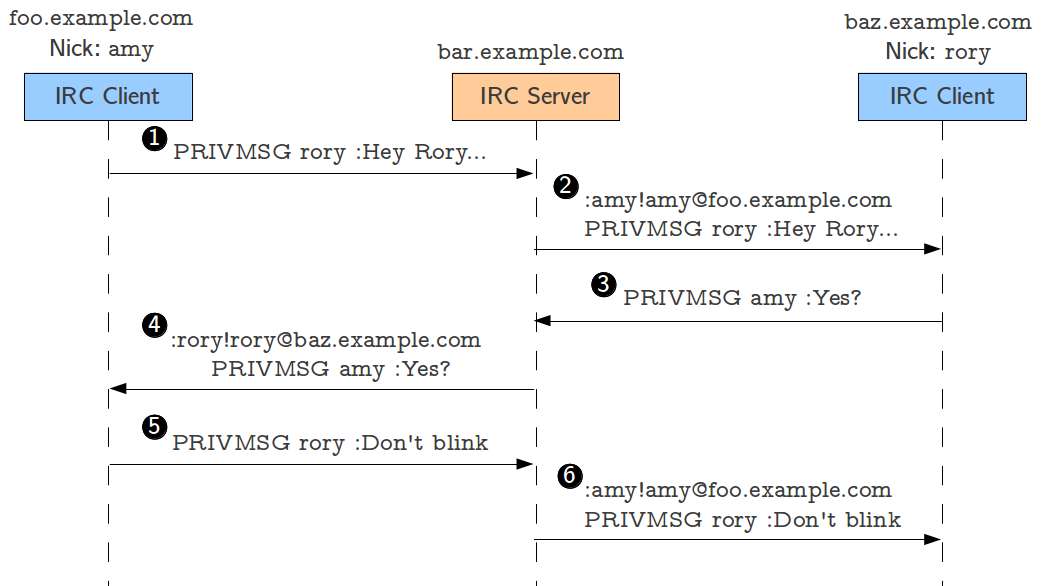
\includegraphics[width=1\textwidth]{privmsg.png}
\caption{Sending a message to another user}
\label{fig:privmsg}
\end{center}
\end{figure}

Once several users are connected, it is possible for them to send messages to each other, even in the absence of channels. In fact, most of Project 1b will focus on implementing messaging between users, whereas Project 1c will focus on adding support for channels.

To send a message to a specific nick, a user must send a \texttt{PRIVMSG} to the server. Figure~\ref{fig:privmsg} shows two users, with nicks \texttt{amy} and \texttt{rory}, exchanging three messages. In message 1, user \texttt{amy} sends a message to \texttt{rory}. The parameters for \texttt{PRIVMSG} are very simple: the first parameter is the nick of the user the message is intended for, and the second parameter is the message itself.

When the server receives that message, and assuming there is a \texttt{rory} user, it will forward the message to the IRC client that is registered with that nick. This is done in message 2, and notice how it is simply a verbatim copy of message 1, but prefixed with \texttt{amy}'s full client identifier (otherwise, the recipient IRC client would have no idea who the message was from). Messages 3 and 4 show a similar exchange, except going from \texttt{rory} to \texttt{amy}, and messages 5 and 6 show another message going from \texttt{amy} to \texttt{rory}.

Notice how all messages are \emph{relayed} through the IRC server (hence the name of the protocol: Internet Relay Chat). Non-relayed messaging is not supported in the IRC specification, and we will not be implementing such a functionality in this project. However, there are two extensions to IRC (CTCP, the Client-to-Client Protocol, and DCC, Direct Client-to-Client) that are the \emph{de facto} standard for non-relayed chat on IRC. Most IRC servers and clients support these extensions, even though they have never been formally specified as an RFC (the closest thing to a specification is this document: \url{http://www.irchelp.org/irchelp/rfc/ctcpspec.html}).


\subsection{Joining, talking in, and leaving a channel}

\begin{sidewaysfigure}
\begin{center}
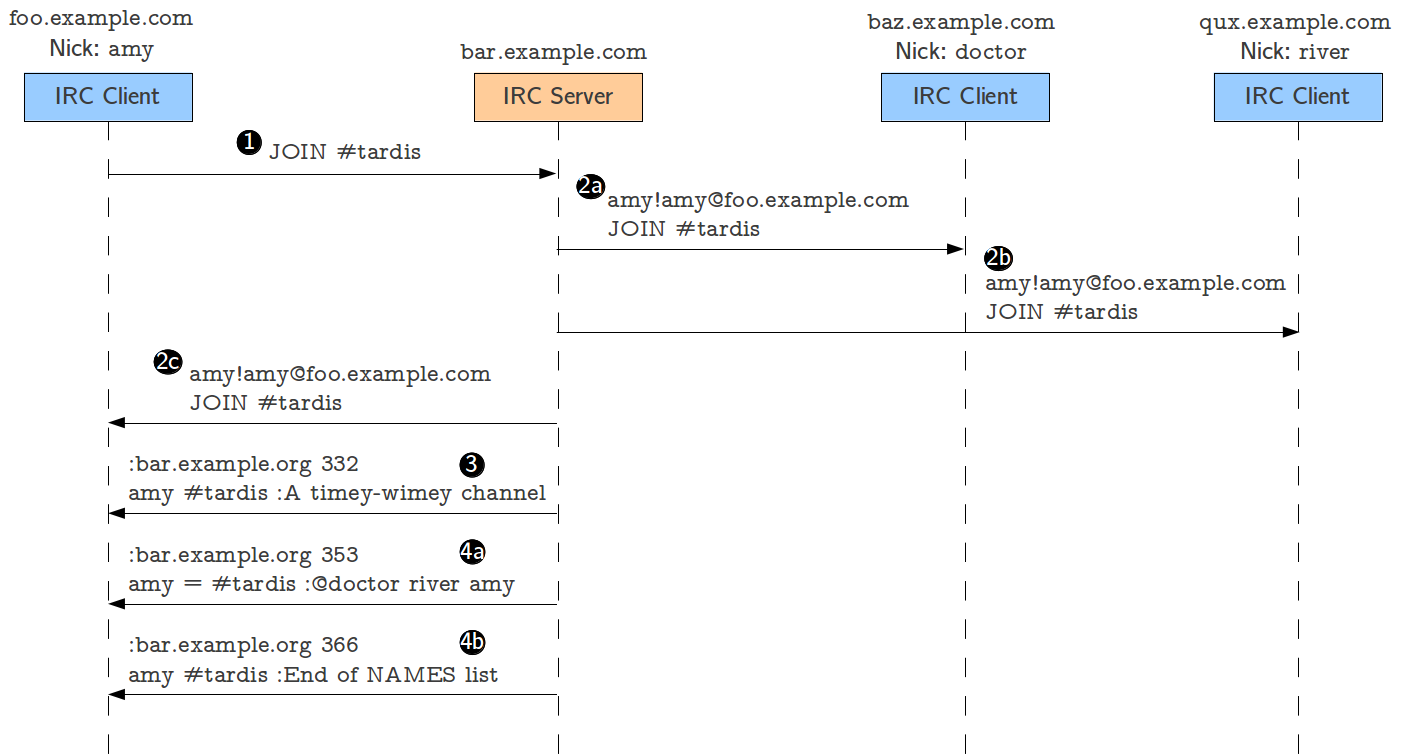
\includegraphics[width=1\textwidth]{channel_join.png}
\caption{Joining a channel}
\label{fig:channel_join}
\end{center}
\end{sidewaysfigure}

Users connected to an IRC server can join existing channels by using the \texttt{JOIN} message. The format of the message itself is pretty simple (its only parameter is the name of the channel the user wants to join), but it results in several replies being sent not just to the user joining the channel, but also to all the users currently in the channel. Figure~\ref{fig:channel_join} shows what happens when user \texttt{amy} joins channel \texttt{\#tardis}, where two users (\texttt{doctor} and \texttt{river}) are already present.

Message 1 is \texttt{amy}'s \texttt{JOIN} message to the server. When this message is received, the server \emph{relays} it to the users who are already in the channel (\texttt{doctor} and \texttt{river}) to make them aware that there is a new user in the channel (messages 2a and 2b). Notice how the relayed \texttt{JOIN} is prefixed with \texttt{amy}'s full client identifier. The \texttt{JOIN} is also relayed back to \texttt{amy}, as confirmation that she successfully joined the channel.

The following messages (3, 4a, and 4b) provide \texttt{amy} with information about the channel. Message 3 is a \texttt{RPL\_TOPIC} reply, providing the channel's \emph{topic} (this is a description of the channel which can be set by certain users; we'll discuss this in detail later). Messages 4a and 4b are \texttt{RPL\_NAMREPLY} and \texttt{RPL\_ENDOFNAMES} replies, respectively, which tell \texttt{amy} what users are currently present in the channel. Notice how the \texttt{doctor} user has an at-sign before his nick; this indicates that \texttt{doctor} is a \emph{channel operator} for channel \texttt{\#tardis}. As we'll see in Project 1c, users can have \emph{modes} that give them special privileges in the server or on individual channels. For example, a channel operator is typically the only type of user that can change the channel's topic.

\begin{sidewaysfigure}
\begin{center}
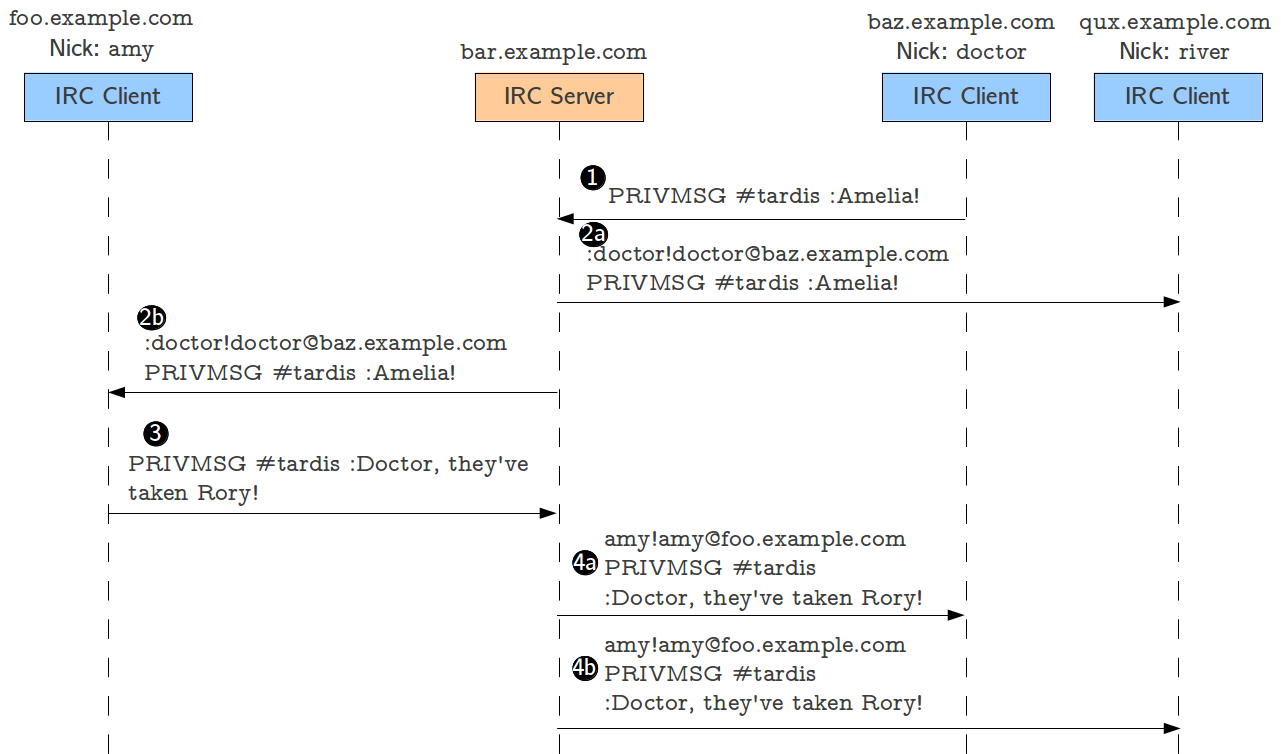
\includegraphics[width=1\textwidth]{channel_privmsg.png}
\caption{Talking in a channel}
\label{fig:channel_privmsg}
\end{center}
\end{sidewaysfigure}

Once a user has joined a channel, sending a message to the channel is essentially the same as sending a message to an individual user. The difference is that the server will relay the message to all the users in the channel, instead of just a single user. Figure~\ref{fig:channel_privmsg} shows two messages being sent to channel \texttt{\#tardis}. First, user \texttt{doctor} sends a \texttt{PRIVMSG} message, specifying the channel as the target (and not a nick, as we saw in Figure~\ref{fig:privmsg}). The server then relays this message to \texttt{river} and \texttt{amy}, prefixing the message with \texttt{doctor}'s full client identifier (messages 1, 2a, and 2b). Similarly, \texttt{amy} sends a message to the channel, which is relayed to \texttt{doctor} and \texttt{river}, prefixed with \texttt{amy}'s full client identifier (messages 3, 4a, and 4b)

\begin{sidewaysfigure}
\begin{center}
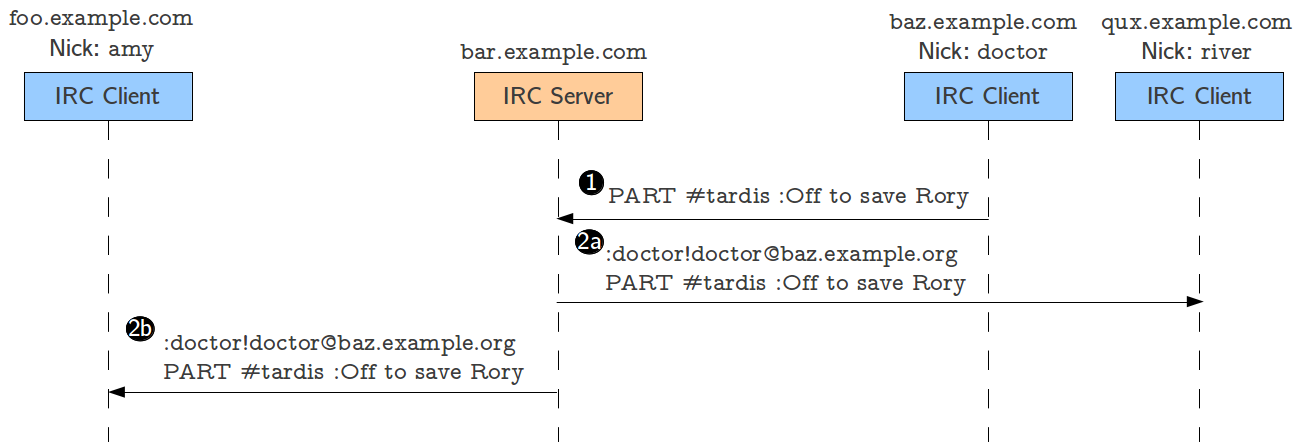
\includegraphics[width=1\textwidth]{channel_part.png}
\caption{Leaving a channel}
\label{fig:channel_part}
\end{center}
\end{sidewaysfigure}

Leaving a channel is accomplished with the \texttt{PART} message, which follows a similar pattern to joining and talking in the channel: the user wishing to leave sends a \texttt{PART} message, and this message is relayed to everyone in the channel so they are aware that the user has left. The server also internally removes that client from the channel, which means he will no longer receive any messages directed to that channel. Figure~\ref{fig:channel_part} shows an example of what this would look like. Notice how the \texttt{PART} message includes two parameters: the channel the users wants to leave, and a ``parting message'' (which is relayed as part of the \texttt{PART} message to all users in the channel).

\section{Getting the \chirc source code}
\label{sec:code}

We are providing some basic code and Makefiles to use as a starting point in your project. It is located in the following GitHub repository:

\begin{center}
\url{https://github.com/uchicago-cmsc23300/chirc}
\end{center}

To download the \chirc code, simply run the following:

\begin{example}
git clone -o upstream git://github.com/uchicago-cmsc23300/chirc.git
\end{example}

This creates a Git repository in directory \texttt{chirc} with a clone of the \chirc repository from GitHub (we will explain what this means in the next section). 

\section{Git in a nutshell}
\label{sec:git}

If you are accustomed to using SVN, we suggest that, at first, you use Git in an ``SVN-like'' manner, without using some of Git's bells and whistles (in fact, you can find a mapping of SVN commands to Git commands in the Git SVN Crash Course: \url{https://git.wiki.kernel.org/articles/g/i/t/GitSvnCrashCourse_512d.html}).

Even so, you should take into account an important difference between Git and SVN: Git is a \emph{distributed} version control system, and SVN is a centralized one. In SVN, there is the notion of a \emph{central} (typically remote) SVN repository that you check out from, check into, and update from. You may have a \emph{working copy} on your local machine, but any time you commit code, the code is committed to the central SVN repository.

Git, on the other hand, has a more general model where, for the same codebase,  there can be multiple repositories, and you have to explicitly state the relationship between them. In practice, it's not uncommon to have one repository that essentially acts as the ``reference'' repository (i.e., the one that is meant to contain the ``authoritative'' version of the code).

So, for example, the \chirc repository on GitHub is simply ``a Git repository''. \texttt{git clone} then created a replica of that repository on your local machine, and this local copy is also just ``a Git repository'' (which happens to be an exact replica of the one on GitHub). This is an important distinction: you are not ``checking out'' code from a server, which is then tied to the server you checked it out from (as is the case with SVN). You are creating a \emph{clone} of an existing Git repository.

Of course, these two repositories are certainly related, and it can be useful to keep track of that relationship. In fact, when cloning a repository, Git will keep track of the clone's \emph{origin} (sometimes called the \emph{upstream} repository). More specifically, a Git repository can track any number of \emph{remote} repositories. Depending on your permissions on those remote repositories, you may be able to \emph{push} changes from your repository to the remote repository (similar, but not exactly, to an \emph{svn commit}), and \emph{fetch} (or \emph{pull}) changes from the remote repository to your repository (e.g., if another developer pushed some changes, and you want to apply them to your own repository, similar to an \texttt{svn update}). 

You can list the remotes for a repository using \texttt{git remote -v}, which should show the following:

\begin{example}
upstream	git://github.com/uchicago-cmsc23300/chirc.git (fetch)
upstream	git://github.com/uchicago-cmsc23300/chirc.git (push)
\end{example}

In this case, you have a single remote called \texttt{upstream} (we specified this name in the \texttt{-o} parameter to \texttt{git clone}). Take into account that \texttt{git remote} simply lists the URLs for the repositories, regardless of whether you have permission to use them or not. In particular, you don't actually have \emph{push} permissions on the \chirc repository on GitHub (only the instructors have \emph{push} permissions on that repository).  

However, you \emph{can} make as many changes as you want to your local clone of the \chirc repository, including making commits. This may sound odd if you're accustomed to SVN, since a commit in SVN always implies ``sending'' that commit to the SVN server. Instead, in Git, you make commits to your local repository. In fact, the only two commands you will need to use at first are just:

\begin{example}
git add \emph{file}
\end{example}

and 

\begin{example}
git commit
\end{example}

Like \texttt{svn add}, the \texttt{git add} command is used to indicate that ``I want to keep track of this file in version control''. However, in Git, it is also used with files that are \emph{already} under version control. More specifically, if you modify a file, you will need to \texttt{git add} it before you can commit it. Once you've added the files that you want to include in a commit, then you run \texttt{git commit}.

Once we provide your team with a private GitHub repository (where you will have both pull \emph{and} push permissions), you will associate this repository with your local repository as an \emph{additional} remote repository. You will then be able to push those changes to that repository, which the instructors will also have access to. We describe how to use this repository in Section~\ref{sec:repo}. 

So, \emph{you do not have to wait until you have that private repository to start working on your project}. Instead, you can work on your local repository (committing changes to your local repository) and, once you get your private GitHub repository, you should push your commits to it (we will explain how to do this in Section~\ref{sec:repo}).

\subsection{Git References}

To learn more about Git, you can find a pretty good introduction here:

\begin{center}
\url{http://learn.github.com/p/intro.html}
\end{center}

If you are familiar with SVN, or other centralized version control systems, you may want to read the Git SVN crash course:

\begin{center}
\url{https://git.wiki.kernel.org/articles/g/i/t/GitSvnCrashCourse_512d.html}
\end{center}

Finally, since we will be setting up a private GitHub repository for you, you may want to work through GitHub's \emph{Set Up Git} guide (\url{help.github.com/set-up-git-redirect/}) to make sure Git is correctly installed on your machine, and set up to work with GitHub.

\section{Building and Testing \chirc}
\label{sec:build}

Once you have the \chirc code, you can build it simply by running Make:

\begin{example}
make
\end{example}

This will generate an executable called \texttt{chirc} that accepts two parameters: \texttt{-p} and \texttt{-o}. The former is used to specify the port on which the server will listen, and the latter to specify the ``operator password''. You need to run the executable with at least the \texttt{-o} option, although this option will not be relevant until Project 1c. For example:

\begin{example}
./chirc -o foobar
\end{example}

The provided code, however, doesn't do anything other that process the command-line parameters. You should nonetheless verify that it builds and runs correctly.

To modify the code, you should \emph{only} add files to the \texttt{src/} directory. Take into account that, if you add additional \texttt{.c} files, you will need to modify the \texttt{src/Makefile} file so they will be included in the build (more specifically, you will need to include a new object file in the \texttt{OBJS} variable).

The provided code also includes a number of automated tests that will be used to verify the correctness of your implementation. You can run all the tests by running the following:

\begin{example}
make tests
\end{example}

For each test that fails, \texttt{make tests} will print the error that caused the test to fail. This output may not be too useful when you first start running the test (and most of the tests will be failing). So, to run a single test, just run the following:

\begin{example}
make singletest TEST=\emph{testname}
\end{example}

The test names are printed when a test fails in \texttt{make tests}. For example, if you see the following:

\begin{example}
======================================================================
ERROR: test_connect_basic1 (tests.test_connection.BasicConnection)
----------------------------------------------------------------------
\emph{. . .   error description   . . .}
\end{example}

You can run just that test by running the following:

\begin{example}
make singletest TEST=\emph{test\_connect\_basic1}
\end{example}

Also, \texttt{make singletest} does not suppress the output of the \texttt{chirc} executable, which will allow you to see any useful logging messages before the test fails.

You can also generate an HTML report that provides a summary of successful and failed tests in a way that is easier to browse. Just run the following:

\begin{example}
make htmltests
\end{example}

This will write a brief summary to the console, and a more detailed report to \texttt{report.html}. 


\section{Using your GitHub repository}
\label{sec:repo}

Once you have formed a group for your project, the instructor will create a private repository for you on GitHub (you will need a GitHub account to access the repository; you will receive instructions about this when the time comes to create your GitHub repository). Only the students in your group will have access to that repository. It will be located in a URL of the following form (the instructor will send you the exact URL when the repository is created):

\begin{center}
\url{https://github.com/uchicago-cmsc23300-students/GROUP_NAME}
\end{center}

This is the repository that the graders will collect your project from. To push the commits from your local Git repository to it, you must set it up as a remote repository. You can do this by running the following:

\begin{example}
git remote add origin git@github.com:uchicago-cmsc23300-students/GROUP_NAME.git
\end{example}

This means your repository now has \emph{two} remotes. \texttt{git remote -v} will now show this:

\begin{example}
upstream	git://github.com/uchicago-cmsc23300/chirc.git (fetch)
upstream	git://github.com/uchicago-cmsc23300/chirc.git (push)
origin 		git@github.com:uchicago-cmsc23300-students/GROUP_NAME.git (fetch)
origin 		git@github.com:uchicago-cmsc23300-students/GROUP_NAME.git (push)
\end{example}

To push all the changes in your local repository to your GitHub repository, just run the following:

\begin{example}
git push origin master
\end{example}

Take into account that, to be able to run this command (which will write to your GitHub repository), you must be authorized to access your GitHub repository from your machine. This is done by adding your SSH key to your GitHub account. You can find instructions on how to do this here: \url{help.github.com/set-up-git-redirect/}.

Furthermore, you can modify the \texttt{.git/config} file so that the default remote is \texttt{origin}, instead of \texttt{upstream} (the read-only repository with the original code). Just make the following change:

\begin{example}
[branch "master"]
	remote = \emph{\textbf{origin}}
	merge = refs/heads/master
\end{example}

This will allow you to push just by running this:

\begin{example}
git push
\end{example}

Finally, if there are any changes in the upstream repository (the one with the original code; e.g., if the instructors find a bug in the code and fix it), you can pull those changes into your repository by running the following:

\begin{example}
git pull upstream master
\end{example}

\pagebreak

\section{Grading}
\label{sec:grading}

For each part of the project, 50\% of the project grade will be determined by the number of automated tests your solution passes successfully, as determined by running \texttt{make tests}. We will use the exact same tests provided in the upstream repository (i.e., there are no additional secret tests that only the graders have access to), and we will let you know what tests will be used specifically for each project part. So, if your solution passes 90\% of the tests before the deadline, you can be certain that you will get at least 45 out of 100 points (i.e., 90\% of 50).

The remaining 50\% of the project grade will be determined by the ``design'' of your code. We will read through your code and check whether you used the appropriate data structures, synchronization primitives, etc. in the various components of your solution. In our experience, the ``design'' grade is typically very similar to the ``tests'' grade so, if you pass 90\% of the tests, it is likely you will get a ``design'' grade in that vicinity. However, the type of feedback you get for this grade is more detailed (instead of a list of automated tests that you pass/fail).

In the specification of what you must do in each project, each part is accompanied by a number of points (e.g., \points{10}). This refers to the design points for that specific part. The amount of points for the automated tests will be roughly, but not exactly, the same (see the report generated by \texttt{make htmltests} for the exact points allocated to each automated test).

\section{Tips}
\label{sec:tips}

\begin{itemize}
\item \emph{Don't be intimidated by the length of the project specification}. The main reason the remaining sections are long is to carve out exactly what part of the IRC specification you have to focus on. You will actually be implementing a fairly small subset of the specification.
\item Similarly, take into account that the division of points is not proportional to the amount of effort required to obtain those points. The points are distributed in such a way that a reasonable amount of work should produce a \emph{good} implementation that will get you roughly 75\% of the points (and will place you in the B range). If you want to produce an \emph{excellent} implementation (placing you in the A range), you will have to go the extra mile to obtain the final 25\% of the points.
\item Your implementation will require using data structures to store collections of users, channels, etc. We do not expect you to implement a data structure from scratch. The instructors' reference implementation uses the SimCList library (\url{http://mij.oltrelinux.com/devel/simclist/}), and we suggest you use it too.
\item As you read the remainder of this document and the IRC specification itself, you'll notice that the same patterns come up over and over. In a sense, your server is just a piece of software that transforms IRC messages into other IRC messages (altering the state of the server in the process). So, before you start tackling individual tests, we suggest you read through the whole document and design your server in such a way that it is easy for you to (1) parse incoming messages, (2) add support for new messages, (3) manipulate the state of the server (e.g., ``create a new channel'', ``add a new user to this channel'', etc.), and (4) construct outgoing messages. Doing so can pay off handsomely later on, even if you spend the first few days feeling like you're not making any progress towards actually earning points.
\item If you're unclear about how your server is meant to behave in some cases (specially the more obscure corner cases), take into account that there are literally hundreds of production IRC servers on the Internet that you can log into to test how they've interpreted the IRC specification. We suggest using Freenode servers, which you can log into simply by running:

\begin{example}
telnet irc.freenode.net 6667
\end{example}

\item Similarly, you can also test your implementation with an existing IRC client. We recommend using \texttt{irssi} (\url{http://irssi.org/}), which is installed on the Maclab Linux machines.
\item Finally, it can sometimes be useful to take a peek at the exact messages that are being exchanged between a client and your server. You can use network sniffers like \texttt{tcpdump} and Wireshark. The console version of Wireshark, \texttt{tshark} can be useful to debug the automated tests. In particular, you can capture the traffic of a test (run with \texttt{make singletest}) by running \texttt{tshark} like this:

\begin{example}
tshark -i lo \textbackslash
       -d tcp.port==7776,irc -R irc -V -O irc -T fields -e irc.request -e irc.response \textbackslash
       tcp port 7776
\end{example}

Note that the automated tests use port 7776 to avoid conflicts with the default IRC port (6667), in case you have a server running separately from the tests.

If you run the above during test \texttt{test\_connect\_basic1}, you should see the following:

\begin{example}
NICK user1	
USER user1 * * :User One	
	:haddock 001 user1 :Welcome to the Internet Relay Network user1!user1@localhost.localdomain
	:haddock 002 user1 :Your host is haddock, running version chirc-0.1
	:haddock 003 user1 :This server was created 2012-01-02 13:30:04
	:haddock 004 user1 haddock chirc-0.1 ao mtov
	:haddock 251 user1 :There are 1 users and 0 services on 1 servers
	:haddock 252 user1 0 :operator(s) online
	:haddock 253 user1 0 :unknown connection(s)
	:haddock 254 user1 0 :channels formed
	:haddock 255 user1 :I have 1 clients and 1 servers
	:haddock 422 user1 :MOTD File is missing
\end{example}

Take into account that the automated tests close the connection as soon as the test has passed, which means sometimes some messages will not be sent. For example, in this specific test, \texttt{tshark} may not capture any messages after the \texttt{001} reply.
\end{itemize}


\pagebreak


\section{Project 1a \points{50}}
\label{sec:proj1a}

This first project is meant as a warm-up exercise to get reacquainted with socket programming. You must implement an IRC server that implements the \texttt{NICK} and \texttt{USER} messages only well enough to perform a \emph{single} user registration as shown in Figure~\ref{fig:connect}. Take into account that a barely minimal server that meets these requirements, and passes the automated tests for this project, can be written in roughly 50 lines of C code (in fact, we will \emph{give you} those 50 lines of code). However, although this kludgy solution will get you a perfect score on the tests, it will earn you a zero on the design grade.

So, you should start implementing your solution with the requirements of the rest of the project in mind. More specifically, your solution to Project 1a should meet the following requirements:

\begin{itemize}
\item \points{12.5} You must send the \texttt{RPL\_WELCOME} \emph{only} after the \texttt{NICK} and \texttt{USER} messages have been received.
\item \points{25} You must take into account that you may get more or less than one full message when you read from a socket. You may not solve this problem by reading one character at a time from the socket.
\item \points{12.5} Your solution must parse the nick and username from the \texttt{NICK} and \texttt{USER} messages, and compose the correct \texttt{RPL\_WELCOME} reply.
\end{itemize}

Although not required for this project, you should take into account that the remaining two parts of the project will involve adding support for additional messages and replies. As we mentioned in Section~\ref{sec:tips}, any time you spend writing a message parser and constructor (that works with more than just \texttt{NICK} and \texttt{USER}) will be time well spent. However, if your solution to Project 1a takes some shortcuts by assuming that you will only be dealing with the \texttt{NICK} and \texttt{USER} messages and the \texttt{RPL\_WELCOME} reply, you will not be penalized for it.

Your server must be implemented in C, and must use sockets. There should be no need for you to use pthreads at this point.

\pagebreak

\section{Project 1b \points{100}}
\label{sec:proj1b}

In this part of the project, your main goal will be to allow users to send messages to each other (as seen in Section~\ref{sec:privmsg}). You will also implement a couple extra messages that will make your server compliant enough to test with existing IRC clients.

Since you will be supporting multiple users, you will now have to spawn a new thread for each user that connects to your server. This, in turn, may result in race conditions in your code. You must identify the shared resources in your server, and make sure they are protected by adequate synchronization primitives.

The messages you have to implement are presented in suggested order of implementation. Nonetheless, once you've implemented Connection Registration, the remaining messages are mostly independent of each other.

\subsection{Connection Registration \points{40}}

Implement connection registration, as described in \RFCsection{2812}{3.1}, with the following exceptions:

\begin{itemize}
\item You must implement the \texttt{NICK}, \texttt{USER}, and \texttt{QUIT} messages. You must \emph{not} implement the \texttt{PASS}, \texttt{SERVICE}, or \texttt{SQUIT} messages. You do not need to implement the \texttt{OPER} and \texttt{MODE} messages yet (you will implement them in Project 1c).
\item In the \texttt{NICK} message, you are only expected implement the \texttt{ERR\_NICKNAMEINUSE} reply.
\item You can ignore the \texttt{<mode>} and \texttt{<unused>} parameters of the \texttt{USER} message.
\item In the \texttt{USER} message, you are only expected to implement the \texttt{ERR\_ALREADYREGISTRED} reply.
\item After a connection has been registered, the \texttt{RPL\_WELCOME} reply must be followed by the \texttt{RPL\_YOURHOST}, \texttt{RPL\_CREATED}, \texttt{RPL\_MYINFO} replies (in that order). For the \texttt{RPL\_MYINFO} reply, the user modes are \texttt{ao} and the channel modes are \texttt{mtov}.
\item The \texttt{ERROR} message sent in reply to a \texttt{QUIT} must include this error message: 

\begin{quote}
\texttt{Closing Link: \textrm{\emph{hostname}} (\textrm{\emph{msg}})}
\end{quote}

\emph{hostname} is the user's hostname. \emph{msg} is the \texttt{<Quit Message>} parameter provided in the \texttt{QUIT} message. If none is provided, the default is \texttt{Client Quit}
\end{itemize}

\noindent Take into account the following:

\begin{itemize}
\item The \texttt{NICK} and \texttt{USER} messages can be received in any order, and a connection is not \emph{fully} registered until both messages have been received (and neither contain any errors)
\item The \texttt{NICK} command can also be used \emph{after} the connection registration to change a user's nick.
\item You can safely skip the \texttt{QUIT} command and revisit it later, as no other commands depend on it.
\item Most IRC servers send the replies corresponding to the \texttt{MOTD} and \texttt{LUSER} messages after the welcome messages are sent. Most of our tests expect this but, until you implement \texttt{MOTD} and \texttt{LUSER}, you can get away with simply sending the following replies verbatim:

\begin{example}
:hostname 251 user1 :There are 1 users and 0 services on 1 servers
:hostname 252 user1 0 :operator(s) online
:hostname 253 user1 0 :unknown connection(s)
:hostname 254 user1 0 :channels formed
:hostname 255 user1 :I have 1 clients and 1 servers
:hostname 422 user1 :MOTD File is missing
\end{example}

This will be enough to pass the connection registration tests (they check that the correct replies are sent, but don't actually check whether they contain accurate information).

\end{itemize}

\subsection{\texttt{PRIVMSG} and \texttt{NOTICE} \points{30}}

Implement messaging between users, as described in \RFCsection{2812}{3.3}, with the following exceptions:

\begin{itemize}
\item The only supported \texttt{<msgtarget>} is nicknames.
\item You must only implement the \texttt{ERR\_NOSUCHNICK} reply.
\end{itemize}

\noindent Take into account the following:

\begin{itemize}
\item If user \texttt{user1} sends a sequence of \texttt{PRIVMSG} messages to \texttt{user2}, then \texttt{user2} \emph{must} receive them in the same order that \texttt{user1} sent them.
\item If users \texttt{user1} and \texttt{user2} each send a single message to \texttt{user3}, the messages are not expected to arrive in the same order that \texttt{user1} and \texttt{user2} sent them. 
\end{itemize}

\subsection{\texttt{PING} and \texttt{PONG} \points{2.5}}

Implement the \texttt{PING} and \texttt{PONG} commands, as described in \RFCsection{2812}{3.7.2} and \RFCsection{2812}{3.7.3}, with the following exceptions:

\begin{itemize}
\item You can ignore the parameters in \texttt{PING}, and simply send the \texttt{PONG} response to the client that sent the \texttt{PING} message.
\item You must silently drop any \texttt{PONG} messages you receive (do \emph{not} send a \texttt{ERR\_UNKNOWNCOMMAND} reply)
\end{itemize}

\noindent Take into account the following:

\begin{itemize}
\item Implementing \texttt{PING} and \texttt{PONG} is essential to testing your server with real IRC clients. IRC clients will sent \texttt{PING} messages periodically and, if they do not receive a \texttt{PONG} message back, they will close the connection.
\end{itemize}

\subsection{\texttt{MOTD} \points{5}}

Implement the \texttt{MOTD} command, as described in \RFCsection{2812}{3.4.1}, with the following exceptions:

\begin{itemize}
\item You can ignore the \texttt{<target>} parameter.
\end{itemize}

\noindent Take into account the following:

\begin{itemize}
\item Your server should read the ``Message Of The Day'' from a file called \texttt{motd.txt} in the directory from where you ran the server.
\item If the file does not exist, you must return a \texttt{ERR\_NOMOTD} reply.
\end{itemize}


\subsection{\texttt{LUSERS} \points{10}}

Implement the \texttt{LUSERS} command, as described in \RFCsection{2812}{3.4.2}, with the following exceptions:

\begin{itemize}
\item You can ignore the \texttt{<mask>} and \texttt{<target>} parameters.
\item You must return the replies in the following order: \texttt{RPL\_LUSERCLIENT}, \texttt{RPL\_LUSEROP}, \texttt{RPL\_LUSERUNKNOWN}, \texttt{RPL\_LUSERCHANNELS}, \texttt{RPL\_LUSERME}
\item You do not need to support the \texttt{ERR\_NOSUCHSERVER} reply
\end{itemize}

\noindent Take into account the following:

\begin{itemize}
\item You must send the replies even when they are reporting a zero value (i.e., ignore this from \RFCsection{2812}{5.1}: ``When replying, a server MUST send back RPL\_LUSERCLIENT and RPL\_LUSERME. The other replies are only sent back if a non-zero count is found for them.'') 
\item An ``unknown connection'' is any connected client that isn't fully registered (i.e., any client that hasn't successfully sent \texttt{NICK} and \texttt{USER}).
\item The number of users in the \texttt{RPL\_LUSERCLIENT} reply is the number of registered users (i.e., all open connections, minus unknown connections).
\item The number of clients in the \texttt{RPL\_LUSERME} reply is the total number of connections, including unknown connections.
\end{itemize}

\subsection{\texttt{WHOIS} \points{10}}

Implement the \texttt{WHOIS} command, as described in \RFCsection{2812}{3.6.2}, with the following exceptions:

\begin{itemize}
\item The command must accept a single parameter: a nick (i.e., there is only a single \texttt{<mask>}, and it must be a nick; ignore the \texttt{<target>} parameter)
\item You must only send back the following replies, in this order: \texttt{RPL\_WHOISUSER}, \texttt{RPL\_WHOISSERVER}, \texttt{RPL\_ENDOFWHOIS}. 
\item You must supply a value for parameter \texttt{<server info>} in \texttt{RPL\_WHOISSERVER}, but we won't be checking its contents.
\item You must support the \texttt{ERR\_NOSUCHNICK} reply.
\end{itemize}

\noindent Take into account the following:

\begin{itemize}
\item You will be implementing \texttt{RPL\_WHOISOPERATOR}, \texttt{RPL\_WHOISCHANNELS}, and \texttt{RPL\_AWAY} in Project 1c.
\end{itemize}

\subsection{\texttt{ERR\_UNKNOWNCOMMAND} \points{2.5}}

If your server receives any message not described here (or in Project 1c), you must return a \texttt{ERR\_UNKNOWNCOMMAND} reply.

\pagebreak

\section{Project 1c \points{100}}
\label{sec:proj1c}

In this part of the project, your main goal will be to add support for channels and modes. You will now have to deal with the fact that messages may be relayed to multiple users, sometimes across multiple channels. 

The parts of this project are presented in suggested order of implementation. Nonetheless, once you've implemented channels (\texttt{JOIN}, \texttt{PART}, and sending messages to channels), implementing modes and the remaining messages are all fairly independent of each other.

\subsection{\texttt{JOIN} \points{15}}

Implement the \texttt{JOIN} command, as described in \RFCsection{2812}{3.2.1}, with the following exceptions:

\begin{itemize}
\item The command must accept a single parameter: a channel name.
\item You must only support the \texttt{RPL\_TOPIC} and \texttt{RPL\_NAMREPLY} replies.
\end{itemize}

\noindent Take into account the following:

\begin{itemize}
\item You must only send a \texttt{RPL\_TOPIC} reply if the channel has a topic (you will implement the \texttt{TOPIC} message later). Otherwise, that reply is skipped.
\item Although not stated explicitly in \RFCsection{2812}{3.2.1}, the \texttt{RPL\_NAMREPLY} reply must be followed by a \texttt{RPL\_ENDOFNAMES} (as shown in Figure~\ref{fig:channel_join}). Basically, you are sending the same replies generated when a \texttt{NAMES} message (with this channel as a parameter) is received.
\item The first automated tests for \texttt{JOIN} will check that the \texttt{RPL\_NAMREPLY} and \texttt{RPL\_ENDOFNAMES} replies are sent, but won't validate their contents. So, you can get away with just sending the following replies (substituting \emph{\texttt{nick}} with the recipient nick):

\begin{example}
:hostname 353 \emph{nick} = #foobar :foobar1 foobar2 foobar3
:hostname 366 \emph{nick} #foobar :End of NAMES list
\end{example}

Once you implement the \texttt{NAMES} message, you can simply substitute this with a call to the same code that handles the \texttt{NAMES} message. Note that, until you implement \texttt{NAMES} correctly, most IRC clients will show your channels as having the three users in your hardcoded \texttt{NAMES} reply (\texttt{foobar1}, \texttt{foobar2}, and \texttt{foobar3})
\end{itemize}


\subsection{\texttt{PRIVMSG} and \texttt{NOTICE} to channels \points{15}}

Extend your implementation of \texttt{PRIVMSG} and \texttt{NOTICE} from Project 1b to support sending messages to a channel.

Until you implement modes, you will not need to support any additional replies in \texttt{PRIVMSG}. However, take into account the following:

\begin{itemize}
\item Despite its name the \texttt{ERR\_NOSUCHNICK} is also the appropriate reply when a non-existent channel is specified.
\item Users cannot send \texttt{PRIVMSG} and \texttt{NOTICE} messages to channels they have not joined. When this happens, a \texttt{ERR\_CANNOTSENDTOCHAN} reply must be sent back (only in the case of \texttt{PRIVMSG} messages).
\item Once you have implement modes, there may be additional cases where a message will be denied if the user has insufficient privileges to speak on a channel.
\end{itemize}


\subsection{\texttt{PART} \points{10}}

Implement the \texttt{PART} command, as described in \RFCsection{2812}{3.2.2}, with the following exceptions:

\begin{itemize}
\item The command must accept either one parameter (a channel name) or two parameters (a channel name and a parting message)
\item You must only support the \texttt{ERR\_NOTONCHANNEL} and \texttt{ERR\_NOSUCHCHANNEL} replies.
\end{itemize}

\noindent Take into account the following:

\begin{itemize}
\item Once all users in a channel have left that channel, the channel must be destroyed.
\end{itemize}


\subsection{\texttt{TOPIC} \points{10}}

Implement the \texttt{TOPIC} command, as described in \RFCsection{2812}{3.2.4}, with the following exceptions:

\begin{itemize}
\item You only need to support the \texttt{ERR\_NOTONCHANNEL}, \texttt{RPL\_NOTOPIC}, and \texttt{RPL\_TOPIC} replies.
\item You will not need to support the \texttt{ERR\_CHANOPRIVSNEEDED} reply until you implement modes.
\end{itemize}


\subsection{User and channel modes \points{25}}

In IRC, users can have certain \emph{modes} assigned to them. Modes are identified by a single letter, and they are binary: a user either has a mode, or he doesn't. The possible user modes are described in \RFCsection{2812}{3.1.5}, and we will be implementing only the following modes:

\begin{description}
\item[\texttt{a}]- The \emph{away} mode. Users with this mode are considered to be ``away from IRC''. Besides being displayed as such on an IRC client, it will also affect how certain messages directed to a user will be processed.
\item[\texttt{o}]- The \emph{operator} mode. Users with this mode have administrative privileges on the IRC server, and have access to certain commands available only to operators.
\end{description}

The above two modes are global modes: they have effect across the entire server. Users can also have channel-specific modes (or \emph{member status} modes, see \RFCsection{2811}{4.1}). We will be implementing the following member status modes:

\begin{description}
\item[\texttt{o}]- The \emph{channel operator} mode. Users with this mode on a channel have special privileges on that channel.
\item[\texttt{v}]- The \emph{voice} mode. Users with this mode are able to send messages to moderated channels (described below).
\end{description}

Finally, channels themselves can also have modes (see \RFCsection{2811}{4}). We will be implementing the following modes:

\begin{description}
\item[\texttt{m}]- The \emph{moderated} mode. When a channel has this mode, only certain users are allowed to send messages to the channel.
\item[\texttt{t}]- The \emph{topic} mode. When a channel has this mode, only a channel operator can set the channel's topic.
\end{description}

These modes are managed with the \texttt{OPER}, \texttt{MODE}, and \texttt{AWAY} commands. For now, we will focus on the first two.

You must implement the \texttt{OPER} message as described in \RFCsection{2812}{3.1.4}, with the following exceptions:

\begin{itemize}
\item You must only support the \texttt{RPL\_YOUREOPER} and \texttt{ERR\_PASSWDMISMATCH}.
\end{itemize}

Take into account that the password expected by the \texttt{OPER} command is the one specified in the \texttt{-o} command-line parameter to the \texttt{chirc} executable.

You must implement the \texttt{MODE} message as described in \RFCsection{2812}{3.1.5} (for user modes) and \RFCsection{2812}{3.2.3} (for member status and channel modes), with the following exceptions:

\begin{itemize}
\item For user modes:
\begin{itemize}
\item You only need to support two (and only two) parameters: the nick and the mode string. The mode string will always be two characters long: a plus or minus character, followed by a letter.
\item You only need to support the \texttt{ERR\_UMODEUNKNOWNFLAG} and \texttt{ERR\_USERSDONTMATCH} replies.
\item If there are no errors, the reply to the \texttt{MODE} message will be a relay of the message, prefixed by the user's nick and with the mode string in a long parameter. So, if a user sends this message:

\begin{example}
MODE jrandom -o
\end{example}

The reply should be:

\begin{example}
:jrandom MODE jrandom :-o
\end{example}

\end{itemize}

\item For channel modes:
\begin{itemize}
\item When only a single parameter (a channel name) is used, the only error condition you must support is the \texttt{ERR\_USERNOTINCHANNEL} reply. If the command is successful, return a \texttt{RPL\_CHANNELMODEIS} reply.
\item When two parameters (a channel name and a mode string) are used, you must support the following error replies: \texttt{ERR\_CHANOPRIVSNEEDED}, \texttt{ERR\_UNKNOWNMODE}, and \texttt{ERR\_USERNOTINCHANNEL}. If the command is successful, the message is relayed back to the user and to all the users in the channel.
\end{itemize}

\item For member status modes:
\begin{itemize}
\item You only need to support three parameters: the channel, the mode string, and the nick.
\item You must support the following error replies: \texttt{ERR\_CHANOPRIVSNEEDED}, \texttt{ERR\_UNKNOWNMODE}, and \texttt{ERR\_USERNOTINCHANNEL}.
\item If the command is successful, the message is relayed back to the user and to all the users in the channel.
\end{itemize}

\end{itemize}

You must observe the following rules when dealing with modes:

\begin{itemize}
\item The \texttt{OPER} message is the \emph{only} way of gaining operator status (the \texttt{o} user mode). Thus, \texttt{+o} is an invalid mode string when using \texttt{MODE}.
\item The \texttt{a} user mode cannot be toggled using the \texttt{MODE} command. Only the \texttt{AWAY} message can manipulate that mode.
\item When a channel is created (when the first user enters that channel), that user is automatically granted the channel operator mode.
\item In a channel, only a channel operator can change the channel modes.
\item In a channel, only a channel operator can change the member status modes of users in that channel.
\item When a channel has the \texttt{m} mode, only channel operators and users with the \texttt{v} member status can send \texttt{PRIVMSG} and \texttt{NOTICE} messages to that channel. Other users will receive an \texttt{ERR\_CANNOTSENDTOCHAN} reply.
\item When a channel has the \texttt{t} mode, only channel operators can change the channel's topic. Other users will receive a \texttt{ERR\_CHANOPRIVSNEEDED} reply.
\item In terms of permissions, server operators (i.e., with user mode \texttt{o}) are assumed to have the same privileges as a channel operator. However, a server operator \emph{does not} explicitly receive the \texttt{o} member status upon joining a channel (the user will simply have, implicitly, the same privileges as a channel operator).
\end{itemize}

\subsection{\texttt{AWAY} \points{5}}

Implement the \texttt{AWAY} command, as described in \RFCsection{2812}{4.1}. 


\subsection{\texttt{NAMES} \points{5}}

Implement the \texttt{NAMES} command, as described in \RFCsection{2812}{3.2.5}, with the following exceptions:

\begin{itemize}
\item We are not supporting invisible, private, or secret channels, so you can consider that all channels are visible to a user sending the \texttt{NAMES} command.
\item You only need to support \texttt{NAMES} messages with no parameters or with a single parameter.
\begin{itemize}
\item When no parameters are specified, you must return a \texttt{RPL\_NAMREPLY} reply for each channel. Since we are not supporting invisible users,
the final \texttt{RPL\_NAMREPLY} must include the names of all the users who are not on any channel.
\item When a single parameters is specified, that parameter is interpreted to be a channel.
\end{itemize}
\item You do not need to support the \texttt{ERR\_TOOMANYMATCHES} and \texttt{ERR\_NOSUCHSERVER} replies.
\end{itemize}

\noindent Take into account the following:

\begin{itemize}
\item Channels and nicks do not need to be listed in any specific order.
\item When you implement modes, nicks with channel operator privileges on a channel must have their nick prefixed by \texttt{$@$} in the \texttt{RPL\_NAMREPLY} reply. Similarly, nicks with ``voice'' privileges must have their nick prefixed by \texttt{+}.
\end{itemize}


\subsection{\texttt{LIST} \points{5}}

Implement the \texttt{LIST} command, as described in \RFCsection{2812}{3.2.6}, with the following exceptions:

\begin{itemize}
\item You only need to support \texttt{LIST} messages with no parameters (list all channels) or with a single parameter (list only the specified channel).
\item You do not need to support the \texttt{ERR\_TOOMANYMATCHES} and \texttt{ERR\_NOSUCHSERVER} replies.
\end{itemize}

\noindent Take into account the following:

\begin{itemize}
\item Channels do not need to be listed in any specific order.
\item In the \texttt{RPL\_LIST} reply, the \texttt{<\# visible>} refers to the total number of users on that channel (since we are not supporting invisible users, the number of visible users equals the total number of users in the channel).
\end{itemize}


\subsection{\texttt{WHO} \points{5}}

Implement the \texttt{WHO} command, as described in \RFCsection{2812}{3.6.1}, with the following exceptions:

\begin{itemize}
\item If a mask is specified, you only need to support the case where the mask is the name of a channel. If such channel exists, you must return a \texttt{RPL\_WHOREPLY} for each user in that channel.
\item We are not supporting invisible clients so, if no mask is specified (or if \texttt{0} or \texttt{*} is specified as a mask), you must return a \texttt{RPL\_WHOREPLY} for each user in the server that doesn't have a common channel with the requesting client. 
\item You do not need to support the \texttt{o} parameter.
\item You do not need to support the \texttt{ERR\_NOSUCHSERVER} reply.
\end{itemize}

\noindent Take into account the following:

\begin{itemize}
\item When a channel is not specified, the \texttt{<channel>} field in the \texttt{RPL\_WHOREPLY} reply must be set to \texttt{*}.
\item In the \texttt{RPL\_WHOREPLY} reply, the \texttt{<\# visible>} refers to the total number of users on that channel (since we are not supporting invisible users, the number of visible users equals the total number of users in the channel).
\item The \texttt{RPL\_WHOREPLY} must return a series of flags, which is specified as \verb|( "H" / "G" > ["*"] [ ( "@" / "+" ) ]| without explanation (furthermore, the \texttt{>} is a typo, and should be a right parenthesis). The flags must be constructed thusly, in this order:
\begin{itemize}
\item If the user is not away, include \texttt{H} (``here'')
\item If the user is away, include \texttt{G} (``gone'')
\item If the user is an operator, include \texttt{*}
\item If the user is a channel operator, include \texttt{@}
\item If the user has the voice mode in the channel, include \texttt{+}
\end{itemize}
\end{itemize}

\subsection{Updating commands from Project 1b \points{5}}

Update the implementation of the following commands:

\begin{itemize}
\item \texttt{NICK}: When a user sends this message, and the change of nick is successful, it must be relayed to all the channels that user is in.
\item \texttt{QUIT}: When a user sends this message, it must be relayed to all the channels that user is in. Take into account that a \texttt{QUIT} results in that user leaving all the channels he is in.
\item \texttt{WHOIS}: Add support for the \texttt{RPL\_WHOISOPERATOR}, \texttt{RPL\_WHOISCHANNELS}, and \texttt{RPL\_AWAY} replies.
\end{itemize}

\end{document}
